\subsection{Sag}
	Dette afsnit vil indeholde en gennem gang af design, grafisk bruger interface og implentering af Sags activityen til android applikationen
	
	\subsubsection{Design}
	Den activity der står for at vise en sag, er bygget op på samme måde som bl.a. LogInActivity, ud fra MVP. Et klasse diagram for dette kan ses på figur \vref{fig:Klasse diagram for Log Ind Android}.
	Specielt for design af CaseActivity, er der lavet flere forskellige layout som skal vises afhængigt af hvilken status den valgte sag har. Sekvensen for dette kan ses på figur \ref{fig:Sekvensdiagram CaseActivity}.
	
	\begin{figure} [!ht]
		\begin{center}
			\includegraphics[height=10cm]{Android/Billeder/sdCaseActivity}
		\end{center}
		\caption{Sekvensdiagram for layout selection}
		\label{fig:Sekvensdiagram CaseActivity}
	\end{figure}
	
	\pagebreak
	
	\subsubsection{Grafisk Bruger Interface}
	De forskellige layouts til at vise en sag ses nedenfor.	
	\begin{figure} [!ht]
		\begin{center}
			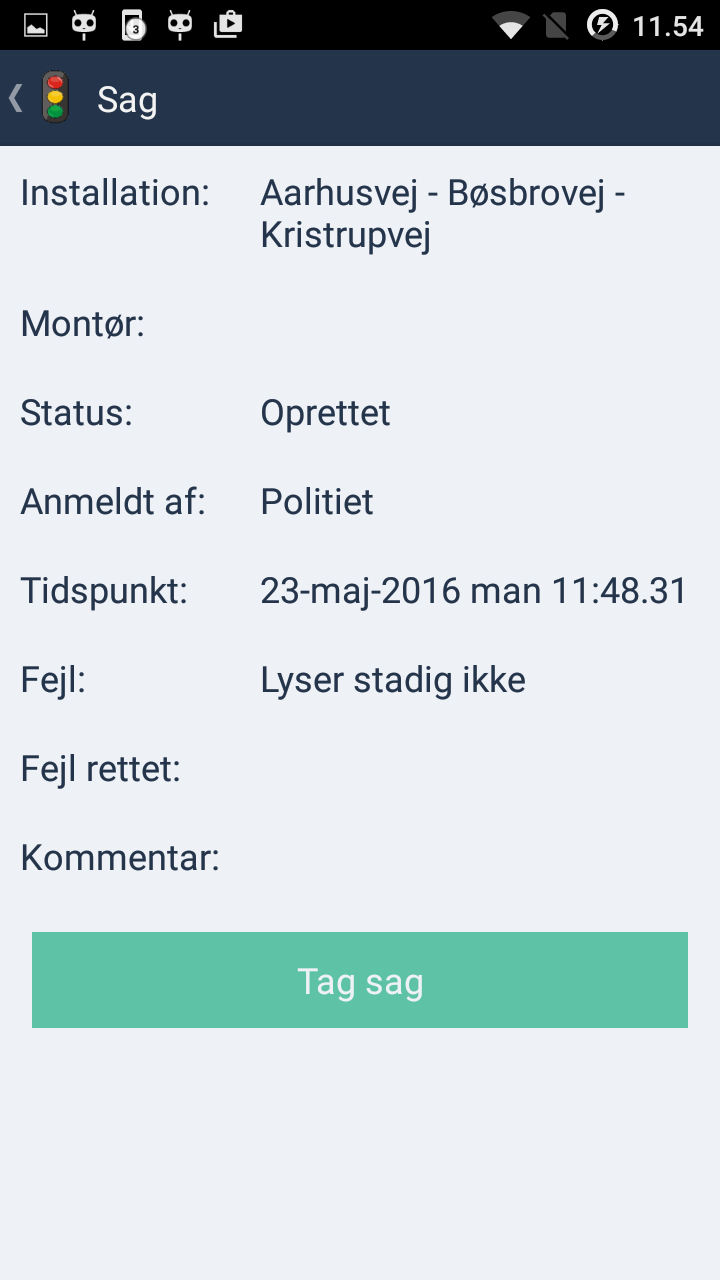
\includegraphics[height=10cm]{Android/Billeder/AndroidSagRod}
		\end{center}
		\caption{Sag der ikke er taget på android applikationen}
		\label{fig:Sag der ikke er taget på android applikationen}
	\end{figure} \\
	Ovenstående billede viser hvordan det vil se ud når en sag endnu ikke er taget, og en montør trykker ind på denne. Her får han en masse info omkring sagen, og til sidst derved muligheden for at tage denne sag.
	\newpage
	
	\begin{figure} [!ht]
		\begin{center}
			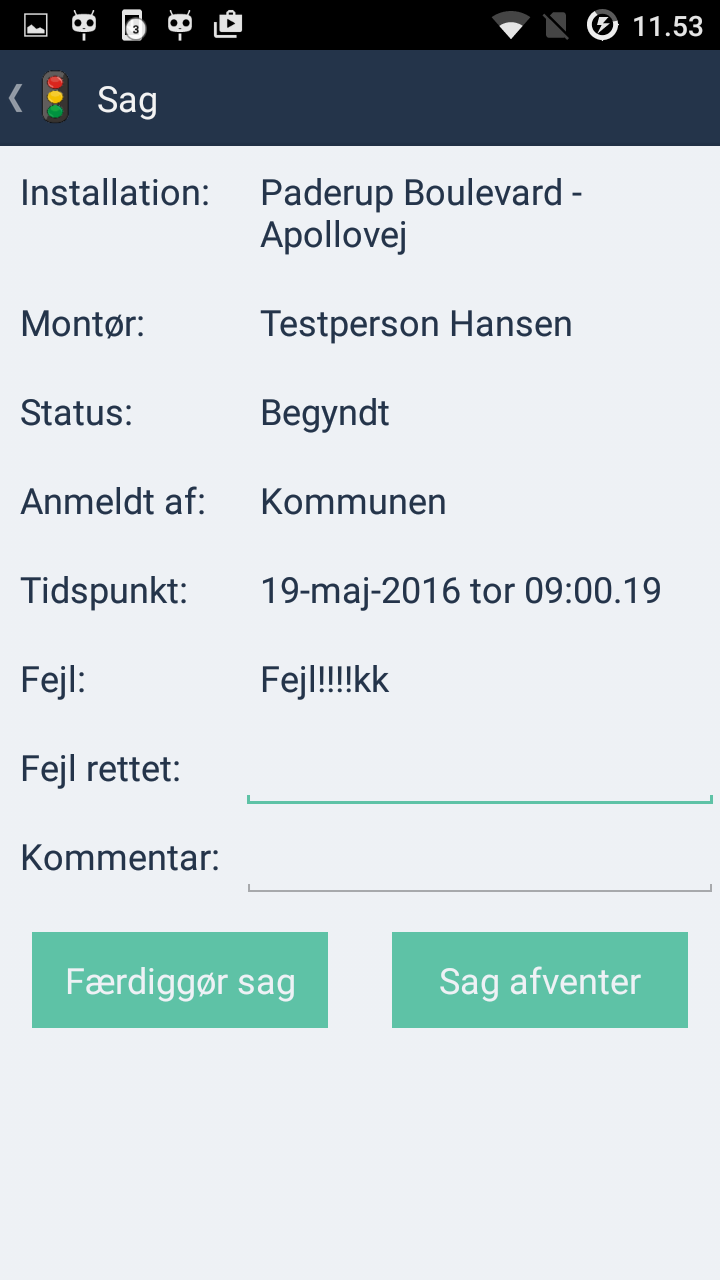
\includegraphics[height=10cm]{Android/Billeder/AndroidSagGul}
		\end{center}
		\caption{Sag der er taget på android applikationen}
		\label{fig:Sag der er taget på android applikationen}
	\end{figure}
	Her ser man en sag når den er taget. Der er info omkring den valgte sag, men der er nu kommet to felter frem, hvor at montøren har mulighed for at skrive kommentar til fejlen og eventuelle andre kommentar. Til sidst kan han så vælge at færdiggør sagen eller sag afventer. Vælges færdiggør sag, lukkes sagen og lyskrydset vises nu som værende kørende igen. Vælges derimod sag afventer betyder dette at reparationene endnu ikke er færdig og der skal en montør ud igen og færdiggøre reparationen.
	
	\pagebreak
	
	\begin{figure} [!ht]
		\begin{center}
			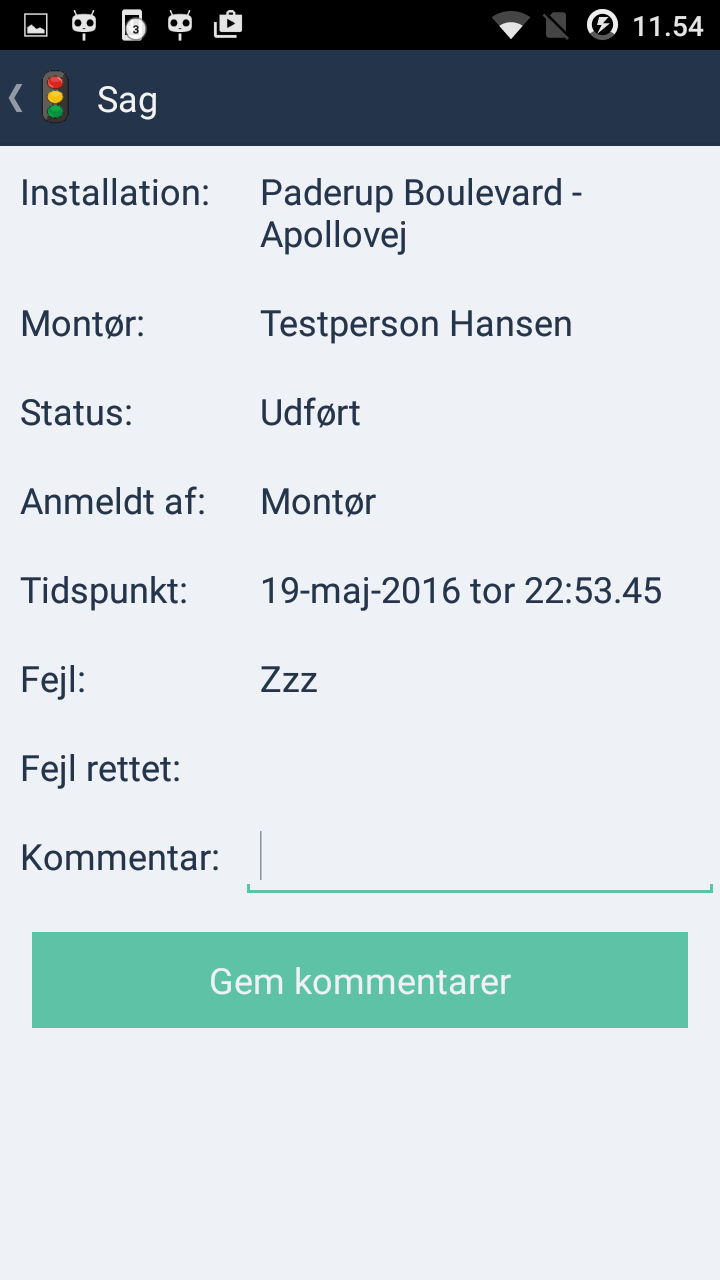
\includegraphics[height=10cm]{Android/Billeder/AndroidSagGron}
		\end{center}
		\caption{Sag der er færdig på android applikationen}
		\label{fig:Sag der er faerdig på android applikationen}
	\end{figure}
	Denne viser hvordan en sag ser ud hvis den er færdiggjort. Man kan som i de andre acticities se info omkring sagen, men det eneste man kan gøre nu er at tilføje en eventuel kommentar.

	
	\subsubsection{Implementering}
	For hvert layout, har presenteren en funktion som bestemmer hvad der skal ske når en pågældende knap i layoutet bliver trykket på. Den valgte sag bliver opdateret med ny status, kommentarer og andet information. Derefter sendes sagen til modellen som sørger for at sagen bliver opdateret i databasen via DAL-laget og API.\\
	Hvis en sag ikke kunne opdateres, giver presenteren viewet besked om at der skal gives en fejlmeddelelse. 
	\pagebreak